\chapter{Use Cases}
\label{ch:Use Cases}

In this chapter, the use cases are discussed.

\subsection{Cross-MANO Framework Interaction}
The MANO frameworks used by every network service provider varies from one another. Scramble with the help of translator and splitter enables the deployment of network services across different frameworks.

For instance: Consider two network service operators using different MANO frameworks. One of them uses Sonata framework \cite{draxler2017sonata} and another operator uses OSM framework \cite{ersue2013etsi}. These frameworks have different NSD schemata. NSD schemata contain VNFs, virtual links, and VNF forwarding graphs and also describes the deployment of a network service. By using a translator and splitter, these NSD schemata can be translated and split into a framework-specific schema. With this, operators can deploy and manage network services across different MANO implementations.

\subsection{Hierarchical Orchestration}
By using MANO adaptor, dynamic instantiation of multiple MANO instances and inter-operability between different MANO frameworks can be achieved. The operator will be able to handle the resources in an efficient manner, as one MANO framework can manage a limited number of service requests, operators can explore options to include additional MANO instances under the existing MANO instance to mitigate the traffic load on a single instance. The resources can be provisioned based on the number of requests. This helps the operator in extending their profitability.

\newpage
\textbf{Actors} : The Network Service Providers who would use features of SCrAMbLE.

\begin{figure}
	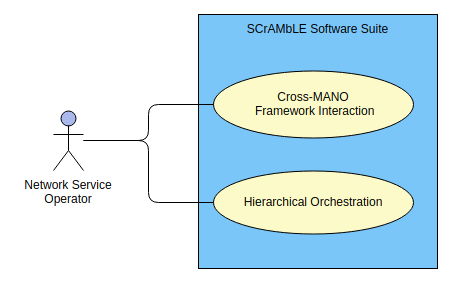
\includegraphics[width=1.0\linewidth]{figures/use-case}
	\caption{Use Case Diagram}
	\label{fig:use-case}
\end{figure}





